\documentclass[12pt, oneside]{article}

\usepackage[letterpaper, scale=0.8, centering]{geometry}
\usepackage{fancyhdr}
\setlength{\parindent}{0em}
\setlength{\parskip}{1em}

\pagestyle{fancy}
\fancyhf{}
\renewcommand{\headrulewidth}{0pt}
\rfoot{{\footnotesize Copyright Mia Minnes, 2024, Version \today~(\thepage)}}

\usepackage{titlesec}

\author{CSE20S24}

\newcommand{\instructions}{{\bf For all HW assignments:} 
These homework assignments may be done individually or in groups of up to 3 students.
Please ensure your name(s) and PID(s)
are clearly visible on the first page of your homework
submission, start each question on a new page, and upload the PDF to Gradescope.
If you're working in a group, {\it submit only one submission per group}: one partner uploads the
submission through their Gradescope account and then adds the other group member(s) to the Gradescope submission
by selecting their name(s) in the ``Add Group Members'' dialog box. You will need to re-add your group member(s)
every time you resubmit a new version of your assignment.

Each homework question will be graded either for
{\bf correctness} (including clear and precise explanations and justifications of all answers) or
{\bf fair effort completeness}. You may collaborate on ``graded for correctness''
questions only with CSE 20 students in your group; if your
 group has questions about a problem, you may ask in drop-in help hours or post a private
post (visible only to the Instructors) on Piazza.  
 For ``graded for completeness''
 questions: collaboration is allowed with any CSE 20 students this quarter; 
 if your group has questions about a problem, you may ask in drop-in 
 help hours or post a public post on Piazza.

All submitted homework for this class must be typed. 
You can use a word processing editor if you like (Microsoft Word, Open Office, Notepad, Vim, Google Docs, etc.) 
but you might find it useful to take this opportunity to learn LaTeX. 
LaTeX is a markup language used widely in computer science and mathematics. 
The homework assignments are typed using LaTeX and you can use the source files 
as templates for typesetting your solutions.

{\bf Integrity reminders}
\begin{itemize}
\item Problems should be solved together, not divided up between the partners. The homework is
designed to give you practice with the main concepts and techniques of the course, 
while getting to know and learn from your classmates.
\item You may not collaborate on homework questions graded for correctness with anyone other than your group members.
You may ask questions about the homework in office hours (of the instructor, TAs, and/or tutors) and 
on Piazza (as private notes viewable only to the Instructors).  
You \emph{cannot} use any online resources about the course content other than the class material 
from this quarter -- this is primarily to ensure that we all use consistent notation and
definitions (aligned with the textbook) and also to protect the learning experience you will have when
the `aha' moments of solving the problem authentically happen.
\item Do not share written solutions or partial solutions for homework with 
other students in the class who are not in your group. Doing so would dilute their learning 
experience and detract from their success in the class.
\end{itemize}

}

\newcommand{\gradeCorrect}{({\it Graded for correctness}) }
\newcommand{\gradeCorrectFirst}{\gradeCorrect\footnote{This means your solution 
will be evaluated not only on the correctness of your answers, but on your ability
to present your ideas clearly and logically. You should explain how you 
arrived at your conclusions, using
mathematically sound reasoning. Whether you use formal proof techniques or 
write a more informal argument
for why something is true, your answers should always be well-supported. 
Your goal should be to convince the
reader that your results and methods are sound.} }
\newcommand{\gradeComplete}{({\it Graded for completeness}) }
\newcommand{\gradeCompleteFirst}{\gradeComplete\footnote{This means you will 
get full credit so long as your submission demonstrates honest effort to 
answer the question. You will not be penalized for incorrect answers. 
To demonstrate your honest effort in answering the question, we 
expect you to include your attempt to answer *each* part of the question. 
If you get stuck with your attempt, you can still demonstrate 
your effort by explaining where you got stuck and what 
you did to try to get unstuck.} }

%\usepackage{tikz}
%\usetikzlibrary{circuits.logic.US,circuits.logic.IEC}

\usepackage{amssymb,amsmath,pifont,amsfonts,comment,enumerate,enumitem}
\usepackage{currfile,xstring,hyperref,tabularx,graphicx,wasysym}
\usepackage[labelformat=empty]{caption}
\usepackage{xcolor}
\usepackage{multicol,multirow,array,listings,tabularx,lastpage,textcomp,booktabs}

% NOTE(joe): This environment is credit @pnpo (https://tex.stackexchange.com/a/218450)
\lstnewenvironment{algorithm}[1][] %defines the algorithm listing environment
{   
    \lstset{ %this is the stype
        mathescape=true,
        frame=tB,
        numbers=left, 
        numberstyle=\tiny,
        basicstyle=\rmfamily\scriptsize, 
        keywordstyle=\color{black}\bfseries,
        keywords={,procedure, div, for, to, input, output, return, datatype, function, in, if, else, foreach, while, begin, end, }
        numbers=left,
        xleftmargin=.04\textwidth,
        #1
    }
}
{}
\lstnewenvironment{java}[1][]
{   
    \lstset{
        language=java,
        mathescape=true,
        frame=tB,
        numbers=left, 
        numberstyle=\tiny,
        basicstyle=\ttfamily\scriptsize, 
        keywordstyle=\color{black}\bfseries,
        keywords={, int, double, for, return, if, else, while, }
        numbers=left,
        xleftmargin=.04\textwidth,
        #1
    }
}
{}

\newcommand\abs[1]{\lvert~#1~\rvert}
\newcommand{\st}{\mid}

\newcommand{\A}[0]{\texttt{A}}
\newcommand{\C}[0]{\texttt{C}}
\newcommand{\G}[0]{\texttt{G}}
\newcommand{\U}[0]{\texttt{U}}

\newcommand{\cmark}{\ding{51}}
\newcommand{\xmark}{\ding{55}}





\title{hw3-circuits-and-logic}
\date{Due: 4/23/24 at 5pm (no penalty late submission until 8am next morning)}
\begin{document}
\maketitle
\thispagestyle{fancy}

{\bf In this assignment}, you will consider how circuits and logic can be used to represent
mathematical claims. You will use propositional operators
to express and evaluate these claims.

{\bf Relevant class material}: Week 2 and Week 3.

You will submit this assignment via Gradescope
(\href{https://www.gradescope.com}{https://www.gradescope.com}) 
in the assignment called ``hw3-circuits-and-logic''.

\instructions

{\bf Assigned questions}

\begin{enumerate}[labelindent=0pt, leftmargin=0pt]
        \item Fixed-width addition.  
        \begin{enumerate}
            \item\gradeCompleteFirst Choose  example width $5$ first summand and width $5$ second summand so that 
            in the  binary fixed-width addition (adding one bit at time, using 
            the usual column-by-column and carry arithmetic, and ignoring the carry 
            from the  leftmost column), we will have that
            \begin{itemize}
            \item[(1)] When interpreting each of the summands and the result in binary fixed-width 5, 
            the result represents the actual value of the sum of the summands {\bf and}
            \item[(2)] when interpreting each of the summands and the sum in sign-magnitude width 5, the result  
            represents the actual value of the sum of the summands {\bf and}
            \item[(3)] when interpreting each of the summands and the sum in 2s complement width 5, the result 
            represents the actual value of the sum of the summands.
            \end{itemize}
            \item\gradeCorrectFirst Choose an example width $5$ first summand and second summand so that 
            in the binary fixed-width addition (adding one bit at time, using 
            the usual column-by-column and carry arithmetic, and ignoring the carry 
            from the  leftmost column), we will have that
            \begin{itemize}
            \item[(1)] When interpreting each of the summands and the result in binary fixed-width 5, 
            the result {\bf does not} represent the actual value of the sum of the summands {\bf and}
            \item[(2)] when interpreting each of the summands and the sum in sign-magnitude width 5, the result  
            {\bf does not} represents the actual value of the sum of the summands {\bf and}
            \item[(3)] when interpreting each of the summands and the sum in 2s complement width 5, the result 
            represents the actual value of the sum of the summands.
            \end{itemize}
            A complete solution will clearly specify each summand and the result of binary fixed-width addition 
            with this choice of summands; will specify  the value of each summand and the result for 
            binary fixed-width 5, 
            sign-magnitude width 5, and 2s complement width 5 (and include calculations connecting with the 
            definitions of these representations to explain these values); and a conclusion connecting
            the calculations to the properties laid out in the question.
        \end{enumerate}    
        \item Circuits. 
        \begin{enumerate}
            \item\gradeComplete Consider the circuit below with inputs $x$ and $y$. 
            Identify a pair of gates that could 
            be switched without changing the input-output table of the circuit.
            If you do, write 
            out the input-output table that results, and briefly explain why 
            this choice of gates works. If there is no such pair of gates, 
            explain why not with reference to the definitions
            of the logic gates.            
        \begin{center}
            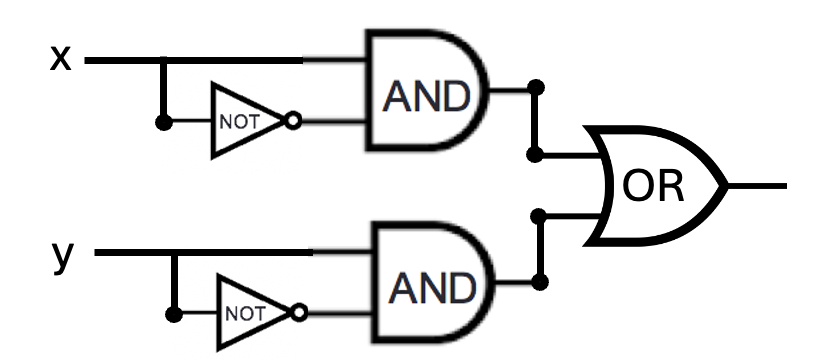
\includegraphics[width=2in]{../../files/circuits-hw3.png}
        \end{center}

        \item\gradeCorrect  Is there a way to fill in the blank portion of 
        the two logic circuits below *with the same gates connected in the same way*
        so that the resulting circuits have the same 
        input-output value *even though* one uses an OR gate at the end and the other 
        uses an XOR gate? If so, design the circuit that would be used, write 
        out the input-output table that results, and briefly explain why your 
        design works. If not, explain why not with reference to the definitions
        of the logic gates.
        \begin{multicols}{2}
            \begin{center}
                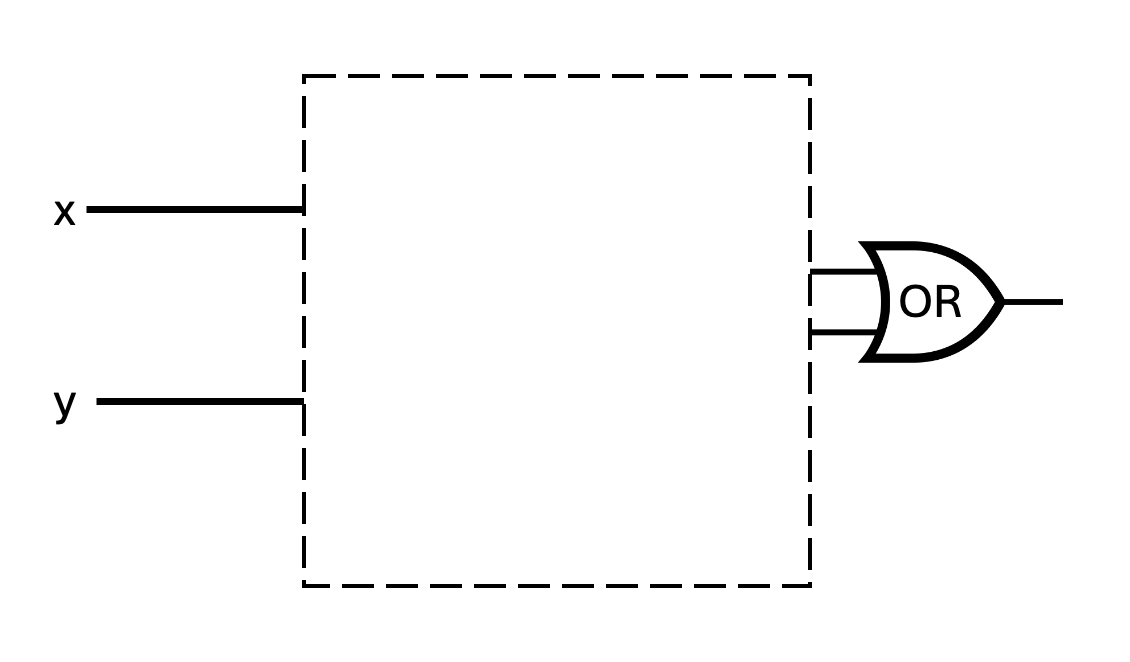
\includegraphics[width=2in]{../../files/circuit-blank-or-hw3.png}
            \end{center}
     
            \begin{center}
                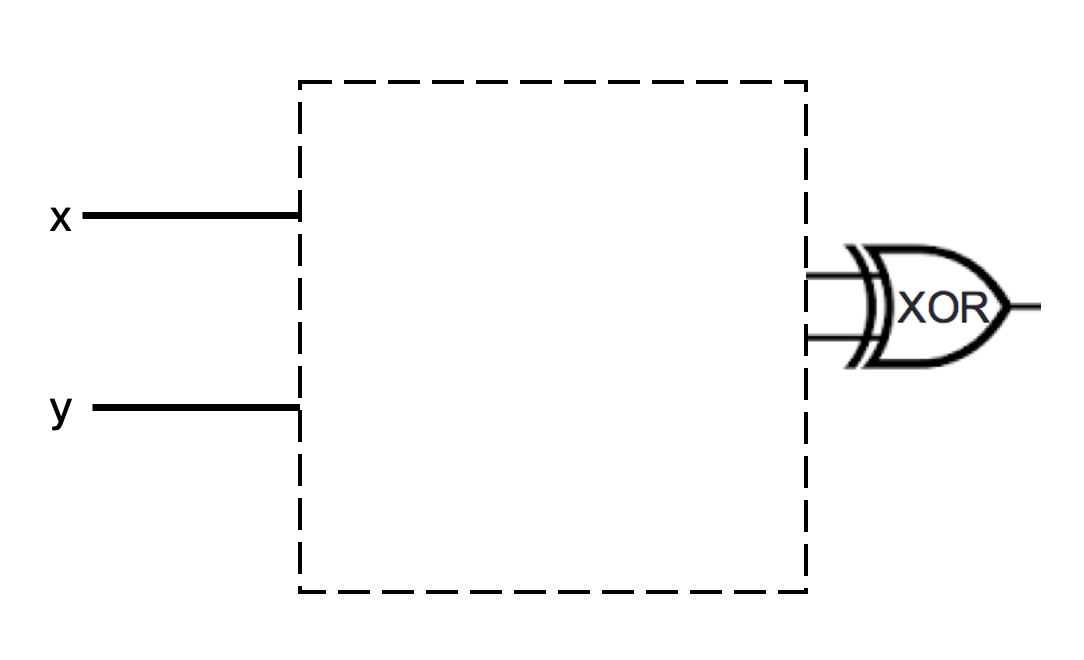
\includegraphics[width=2in]{../../files/circuit-blank-xor-hw3.png}
            \end{center}
        \end{multicols}

    \end{enumerate}
    \newpage
    \item Compound propositions. The set of strings of length $4$ whose characters are $0$s or $1$s is
        the result of four successive set-wise concatenations: $\{0,1\} \circ \{0,1\} \circ \{0,1\}$. Let's call
        this set $X_4$. Consider the function $f: X_4 \to X_4$ defined by
        $$ f(x) = 
        \begin{cases} 
            y &\text{when $(x)_{2,4} < 15$ and $(y)_{2,4} = (x)_{2,4} + 1$}\\
            1111 &\text{when $x = 1111$}
        \end{cases}$$
        for each $x \in X_4$. In other words, we can describe the function as: $f$ takes a string, interprets it as the binary fixed-width $4$
        expansion of an integer, and then adds $1$ to that integer (unless $x$ is already representing
        the greatest integer that can be represented in binary fixed-width $4$) and outputs the binary 
        fixed-width $4$ expansion of the result.
        \begin{enumerate} 
        \item\gradeComplete Fill in the blanks in the following input-output definition table 
        with four inputs $x_3$, $x_2$, $x_1$, $x_0$ and four outputs $y_3$, $y_2$, $y_1$, $y_0$
        so that $f(x_3x_2x_1x_0) = y_3y_2y_1y_0$.
        
        \begin{center}
        \begin{tabular}{cccc|cccc}
        $x_3$ & $x_2$ & $x_1$ & $x_0$ & $y_3$ & $y_2$ & $y_1$ & $y_0$\\
        \hline
        $1$ & $1$ & $1$ & $1$ & $1$ & $1$ & BLANK1 & $1$\\
        $1$ & $1$ & $1$ & $0$ & $1$ & $1$ & $1$ & $1$\\
        $1$ & $1$ & $0$ & $1$ & $1$ & BLANK2 & $1$ & $0$\\
        $1$ & $1$ & $0$ & $0$ & $1$ & $1$ & $0$ & $1$\\
        $1$ & $0$ & $1$ & $1$ & $1$ & $1$ & $0$ & $0$\\
        $1$ & $0$ & $1$ & $0$ & $1$ & $0$ & $1$ & $1$\\
        $1$ & $0$ & $0$ & $1$ & $1$ & $0$ & $1$ & $0$\\
        $1$ & $0$ & $0$ & $0$ & BLANK3& $0$ & $0$ & $1$\\
        $0$ & $1$ & $1$ & $1$ & $1$ & $0$ & $0$ & $0$\\
        $0$ & $1$ & $1$ & $0$ & $0$ & $1$ & $1$ & BLANK4\\
        $0$ & $1$ & $0$ & $1$ & $0$ & $1$ & $1$ & BLANK5\\
        $0$ & $1$ & $0$ & $0$ & $0$ & $1$ & $0$ & $1$\\
        $0$ & $0$ & $1$ & $1$ & $0$ & $1$ & $0$ & $0$\\
        $0$ & $0$ & $1$ & $0$ & $0$ & $0$ & $1$ & $1$\\
        $0$ & $0$ & $0$ & $1$ & $0$ & $0$ & $1$ & $0$\\
        $0$ & $0$ & $0$ & $0$ & BLANK6 & $0$ & $0$ & $1$\\
        \end{tabular}
        \end{center}
  
        \item\gradeCorrect
        Construct an expression (as a compound proposition) for $y_0$ in terms of the inputs 
        $x_3, x_2, x_1, x_0$. Justify your expression by referring to the definition of the logic 
        gates XOR, AND, OR, NOT and the definition of the function $f$. Hint: our work on the half-adder might 
        be helpful.
        \item\gradeCorrect
        Construct an expression (as a compound proposition) for $y_1$ in terms of the inputs 
        $x_3, x_2, x_1, x_0$. Justify your expression by referring to the definition of the logic 
        gates XOR, AND, OR, NOT and the definition of the function $f$. Hint: our work on the half-adder might 
        be helpful.
        \item\gradeComplete Draw a combinatorial circuit corresponding to these compound propositions.
        Remember that the symbols for the inputs will be on the left-hand-side and 
        the symbol for the outputs $y_0$ and $y_1$ will be on the right-hand side. Use gates (draw the appropriate
        shapes and add labels for clarity) and wires to connect the inputs appropriately to give the output.
        \item\gradeComplete Construct expressions (as a compound propositions) for $y_2$ and $y_3$ 
        in terms of the inputs  $x_3, x_2, x_1, x_0$. Are these similar to the expressions for $y_0$ and $y_1$?
        \end{enumerate}
        \item Logical Equivalence. Imagine a friend suggests the following argument to you: ``The compound proposition
        \[
        (x \lor y) \land z
        \]
        is logically equivalent to 
        \[
        x \lor (y \land z)
        \]
        because I can transform one to the other using the following sequence of logical equivalences: 
        \[
           (x \lor y) \land z \equiv
           (x \lor (y \land y)) \land z \equiv
           x \lor ( (y \lor y) \land z) \equiv x \lor (y \land z) 
        \]
        because $y$ is logically equivalent to both $y \land y$ and to $y \lor y$".
        
        \begin{enumerate}
        \item\gradeCorrect Prove to your friend that they made a mistake by giving a truth
        assignment to the propositional variables $x,y,z$ so that 
        the two compound propositions 
        $ (x \lor y) \land z$ and $ x \lor (y \land z)$ have different truth values.
        Justify your choice by evaluating these compound propositions using the definitions of the logical connectives 
        and include enough intermediate steps so that a student in CSE 20 who may be 
        struggling with the material can still follow along with your reasoning.
        
        \item\gradeComplete 
        Help your friend find the problem in their argument by pointing out which step(s) were incorrect.
        
        \item\gradeComplete Give {\bf three} different compound propositions
        that are actually logically equivalent to (and not the same as)
        \[
            (x \lor y) \land z
        \]
        Justify each one of these logical equivalences either by applying a sequence of logical equivalences
        or using a truth table.  Notice that you can use other logical operators (e.g. $\lnot, \lor, \land, \oplus, \to, 
        \leftrightarrow$) 
        when constructing your compound propositions.
     
        {\it Bonus; not for credit (do not hand in)}: How would you translate each of the equivalent compound
        propositions in English? Does doing so help illustrate why they are equivalent?
        \end{enumerate}
        
     
\end{enumerate}
\end{document}
\begin{comment}
\item Functions and algorithms: in this question you'll explore the properties of the (integer) power and logarithm
functions. We'll use some definitions we introduced in class this week, namely the function
$b^i$ with domain $\mathbb{Z}^+ \times \mathbb{N}$ and codomain $\mathbb{N}$ defined recursively by
\begin{align*}    
&\textrm{Basis Step:} \\
&b^0 = 1 \\
&\textrm{Recursive Step:}\\
&\textrm{If } i \in \mathbb{N}, b^{i+1} = b \cdot b^i
\end{align*}
and the algorithm:
%! app: Numbers
%! outcome: number representation

\begin{algorithm}[caption={Calculating integer part of base $b$ logarithm}]
   procedure $logb$($b$,$n$: positive integers with $b > 1$)
   $i$ := $0$
   while $n$ > $b-1$
     $i$ := $i + 1$
     $n$ := $n$ div $b$
   return $i$ $\{ i$ holds the integer part of the base $b$ logarithm of $n\}$
\end{algorithm}


    \begin{enumerate}
    \item\gradeCorrectFirst Choose a positive integer $b$ between $3$ and $6$ (inclusive) and choose a 
    nonnegative integer $i$ between $2$ and $5$ (inclusive). Demonstrate how to calculate 
    the result of the $logb$ algorithm (procedure) when its input is the base $b$ you chose and
    $n = b^i$ (for the $i$ you choose.) 
    A complete answer will include the specific choice of $b$ and $i$, along with 
    trace of the calculations of $b^i$ and the computation of the algorithm, including 
    (clear, correct, complete) calculations for each of the function applications 
    and/or references to definitions and a trace table for algorithm that includes the values of all relevant 
    variables at each iteration (See the annotated Week 2 notes for the level of detail expected
    in a trace of a function application and a trace table).
    \item\gradeCorrect Now we'll go in other order: Demonstrate how to calculate the result of 
    $7^y$ where $y$ is the result of the $logb$ algorithm (procedure) when its input is $b=7$ and $n=30$.
    A complete answer will include clearly labelled 
    traces of the calculations of $b^i$ and the computation of the algorithm, including 
    (clear, correct, complete) calculations for each of the function applications 
    and/or references to definitions and a trace table for algorithm that includes the values of all relevant 
    variables at each iteration (See the annotated Week 2 notes for the level of detail expected
    in a trace of a function application and a trace table).    
    \item\gradeCompleteFirst Logarithms and powers are supposed to ``undo" one another. Explain whether your work in parts (a) and (b)
    supports that idea,  whether you saw anything confusing or surprising about these calculations, and how to explain what you saw.
    \end{enumerate}

\item Base expansions
    \begin{enumerate}
        \item\gradeComplete Pick an integer between $50$ and $1000$ (inclusive) that you (or one of your
        group members) came across at some point this week. 
        In a sentence or two, give some context for why you're choosing this number). 
        Write the base expansion of your chosen number in base $2$ (binary), base $3$ (ternary), base $4$, and base $16$ (hexadecimal).
        \item\gradeCorrect What is the {\bf smallest} width $w$ in which they could write your chosen number in base $8$ (octal) 
        fixed-width $w$? Justify your answer with reference to the definitions of fixed-width expansions and relevant calculations.
        \item\gradeCorrect Express in roster method the set of numbers between $1$ and $2$ (exclusive) that be written without error 
        (full precision)
        in binary fixed width expansion with integer part width $3$ and fractional part width $2$. Justify your answer with 
        reference to the definitions of fixed-width expansions and relevant calculations.
        \item\gradeCorrect Consider the strings of $1$s that have length $3$, $5$, $7$, and $10$.
        Calculate the numbers 
        \begin{itemize}
            \item[] $[111]_{s,3}$
            \item[] $[11111]_{s,5}$
            \item[] $[1111111]_{s,7}$
            \item[] $[1111111111]_{s,10}$
            \item[] $[111]_{2c,3}$
            \item[] $[11111]_{2c,5}$
            \item[] $[1111111]_{2c,7}$
            \item[] $[1111111111]_{2c,10}$
        \end{itemize}
        Justify your answers with specific reference to the definitions of sign-magnitude and $2$s complement expansions and relevant calculations.
        \item \gradeComplete What patterns do you notice in your calculations in part (d)?
    \end{enumerate}

\item Multiple representations

Recall that, mathematically, a color can be represented as a $3$-tuple $(r, g, b)$ 
where $r$ represents the red component, $g$ the green component, $b$ the blue component and where each of $r$, $g$, $b$ must be from the collection $\{x \in \mathbb{N}\mid 0 \leq x \leq 255 \}$.
As an alternative representation, in this assignment
we'll use base $b$ fixed-width expansions to represent colors
as individual numbers (this definition was introduced in this week's Review quiz).

{\bf Definition}: A {\bf hex color} is a nonnegative
integer, $n$, that has a base $16$ fixed-width $6$  expansion
$$n = (r_1r_2g_1g_2b_1b_2)_{16,6}$$ 
where $(r_1r_2)_{16,2}$ is the red
component, $(g_1g_2)_{16,2}$ is the green component, 
and $(b_1b_2)_{16,2}$ is the
blue.

For this question, let's call the set of hex colors $H$. In the Week 2 Review quiz (Question 3d), 
we explored a few different set builder definitions for $H$.

\begin{enumerate}
\item \gradeComplete Rewrite the set builder definition of a set below so that it 
refers to colors rather than numbers: $\{ c \in H \mid c \mod 256 = 0\}$. A complete answer will 
justify the new set builder definition by connection with the definition of hex colors and how it impacts
the colors that satisfy the specific property for this set.
\item \gradeCorrect Rewrite the set builder definition of a set below so that it 
refers to colors rather than numbers: $\{ c \in H \mid c < 65536\}$. A complete answer will 
justify the new set builder definition by connection with the definition of hex colors and how it impacts
the colors that satisfy the specific property for this set.
\item \gradeCorrect In art, we can mix two colors to get a new color. For example, red and blue make 
purple, blue and yellow make green, red and yellow make orange. 
A mathematical definition of {\bf hex color mixing} would be a function with domain $H \times H$
and codomain $H$ where the result of applying this function to an input $(n_1, n_2)$ is the hex color
that results from mixing the hex colors $n_1$ and $n_2$.


\rule{0.5\textwidth}{.4pt}

{\it Sample work for a related question that can be used as reference for the detail expected 
in your answer:} Consider the attempted mathematical definition  $f_1: H\times H \to H$ given by
\[
f_1 (~(n_1, n_2) ~) = n_1 + n_2
\]
We will show that this function is not well-defined so it cannot give a hex color mixing definition. 
The reason it is not well-defined
is that the application of the rule sometimes gives values that are not in the stated codomain. 
To see this, we need an example input to $f_1$ for which the output of the rule is not in $H$.
Here is one such example: $(n_1, n_2) = (~(FFFFFF)_{16,6}, (FFFFFF)_{16,6}~)$. 
This example is in $H \times H$
because $(FFFFFF)_{16,6}$ is a nonnegative integer that has a base $16$ fixed-width $6$ expansion 
so it is a hex color.
We now apply the definition of the rule in $f_1$:
\begin{align*}
f_1 (~(n_1, n_2) ~) &=  f_1 ( (~(FFFFFF)_{16,6}, (FFFFFF)_{16,6}~) ) = (FFFFFF)_{16,6} + (FFFFFF)_{16,6} \\
&= 2 \left( 15\cdot 16^5 + 15\cdot 16^4 + 15 \cdot 16^3 + 15 \cdot 16^2 + 15 \cdot 16^1 + 15 \cdot 16^0 \right) \\
&= 2 \cdot 15 \cdot (1048576 + 65536 + 4096 + 256 + 16 + 1) = 2 \cdot 15 \cdot 1118481 = 33554430
\end{align*}
This is not a hex color because it is greater than or equal to $16^6 = 16777216$, 
so (using the Week 2 notes on which numbers can be represented
with fixed-width expansions) it does not have a hexadecimal {\bf fixed width $6$} expansion.

\rule{0.5\textwidth}{.4pt}

In this question, we'll look at another attempted mathematical definition for hex color mixing. 
We define $f_2: H\times H \to H$ given by
\[
f_2 (~(n_1, n_2) ~) = (n_1 + n_2) \textbf{ div } 2
\]

This is a well-defined function. You do not need to prove this or hand it in, but it's good practice to make 
sure you understand why it's well-defined. Notice that the function application 
\[
f_2 ( ~(~ (FF0000)_{16,6} , (FFFE00)_{16,6} ~)~)
\]
can be calculated as:
\begin{align*}
f_2&(((FF0000)_{16,6}, (FFFE00)_{16,6}))=
 ((FF0000)_{16,6} + (FFFE00)_{16,6})) \textbf{ div } 2\\
&= \big(~ \left(15\cdot16^5 + 15\cdot16^4 + 0\cdot16^3 + 0\cdot16^2 + 0\cdot16^1 + 0\cdot16^0 \right) \\
&~~~~+~
    \left((15\cdot16^5 + 15\cdot16^4 + 15\cdot16^3 + 14\cdot16^2 + 0\cdot16^1 + 0\cdot16^0\right )~\big )\textbf{ div } 2\\
&= (16711680 + 16776704) \textbf{ div } 2 = 33488384 \textbf{ div } 2 = 16744192
\end{align*}
Since this is less than $16^6 = 16777216$, we can represent it using base $16$ fixed-width $6$:.
$$(16744192)_{10} = 15\cdot16^5 + 15\cdot16^4 + 7\cdot16^3 + 15\cdot16^2 + 0\cdot16^1 + 0\cdot16^0 = (FF7F00)_{16,6}$$

Using the web tool \url{https://www.w3schools.com/colors/colors_rgb.asp}, we can verify that $(FF0000)_{16,6}$ is red, 
$(FFFE00)_{16,6}$ is yellow, and $(FF7F00)_{16,6}$ is orange.

Show that $f_2$ does not work as a hex color mixing definition by finding
another ordered pair of hex colors for which the result of applying $f_2$ does not give the expected hex color.
Include the numerical description of each colors you mention, alongside a description of them in English. 
Describe how you know what these colors are
(if you use a web color tool, include its URL in your submission writeup; if not, describe your reasoning).
Justify your 
example with (clear, correct, complete) calculations and/or references to definitions, and connecting them with
the desired conclusion.
\end{enumerate}
\end{enumerate}
\end{comment}